\documentclass[aspectratio=169]{beamer}
\mode<presentation>

% \documentclass[aspectratio=169,handout]{beamer}
% \mode<presentation>
% \setbeameroption{show notes}
% \usepackage{pgfpages}
% \pgfpagesuselayout{6 on 1}[letterpaper,border shrink=5mm]


%Theme and Color of Presentation
\usetheme{CambridgeUS}
\usecolortheme{seahorse}
\useinnertheme{rectangles}

%Colors
% From https://www.utdallas.edu/brand/color-palette/
\definecolor{UTDorange}{RGB}{232,117,0}
\definecolor{UTDgreen}{RGB}{18,71,52}
\definecolor{UTDseafoam}{RGB}{95,244,183}

\setbeamercolor{palette primary}{bg=UTDorange,fg=white}
\setbeamercolor{palette secondary}{bg=UTDgreen,fg=white}
\setbeamercolor{palette tertiary}{bg=UTDorange,fg=white}
\setbeamercolor{palette quaternary}{bg=UTDorange,fg=white}
\setbeamercolor{frametitle}{fg=UTDgreen}
\setbeamercolor{structure}{fg=UTDgreen} % itemize, enumerate, etc
\setbeamercolor{subsection in head/foot}{bg=UTDgreen,fg=white}


%Additional Packages
\usepackage{graphicx}
\usepackage{physics}
\usepackage{amsmath}
\usepackage{setspace}
\usepackage{textpos}
\usepackage{hyperref}
\usepackage{xcolor}

%Additional Settings/Commands
\newcommand{\extraspace}{\vskip 0.5em}

\AtBeginSection[]
{
	\begin{frame}
		\frametitle{Outline}
		\tableofcontents[currentsection]
	\end{frame}
}
%\AtBeginSubsection[]
%{
%	\begin{frame}
%		\frametitle{Outline}
%		\tableofcontents[currentsection,currentsubsection]
%	\end{frame}
%}

%Presentation Info
\title[Frequency Response Analysis]{Introduction to Frequency Response Analysis}
\subtitle{Mechanical System Forced Response, Transfer Functions, and Input-Output Characterization}
\author{Jonas Wagner}
\institute[UTDallas]{The University of Texas at Dallas}
% \date[ME GTF Interview - Fall 2021]{Mechanical Engineering Graduate Teaching Fellowship Teaching Example - Fall 2021}
% Updated since original usage
\date{}

\begin{document}
	
\begin{frame}
	\titlepage
\end{frame}

\addtobeamertemplate{frametitle}{}{%
	\begin{textblock*}{100mm}(.85\textwidth,-1cm)
		
\includegraphics[height=1cm]{Images/UT_Dallas_Logo}
	\end{textblock*}
}

\begin{frame}{Outline}
	\tableofcontents
	\note{

	}
\end{frame}

\section{Background}
\begin{frame}
	\frametitle{Review: Mechanical System Modeling}
	\begin{columns}
		\begin{column}{0.5 \textwidth}
			\[F = m \vb{a} = m \dv{t} \vb{v} = m \dv{t} \qty(\dv{t} \vb{x})\]
			\[
				m \dv{t^2} x(t) 
				= \sum F 
				= f(t) - b \dv{t} x(t) - k x(t)
			\]

			Let $\vb{x} = x(t)$ and $\vb{u} = f(t)$
			\[
				m \ddot{\vb{x}} + c \dot{\vb{x}} + k \va{x} = \vb{u}
			\]
			\[
				\ddot{\vb{x}} 
				= \qty(\frac{-c}{m}) \dot{\vb{x}} + \qty(\frac{-k}{m}) \vb{x} + \qty(\cfrac{1}{m}) \vb{u}
			\]
			\[
				\dv{t} \mqty[
					\dot{\vb{x}}\\ 
					\vb{x}
				 ] = 
				\mqty[
					1 &0\\
					-\frac{c}{m} &-\frac{k}{m}
					] 
				\mqty[
					\dot{\vb{x}}\\
					\vb{x}
				]
				+ \mqty[
					0\\
					\frac{1}{m}
				]
				\mqty[\vb{u}]
			\]
		\end{column}
		\begin{column}{0.375 \textwidth}
			\begin{figure}[]
				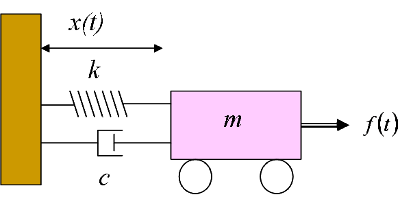
\includegraphics[width=\textwidth]{Images/SpringMassDamper_cartSystem.png}
				Spring Mass Damper System \cite{ctms_engin_umich_SystemModeling}
			\end{figure}
		\end{column}
	\end{columns}
	\note{

	}
\end{frame}

\begin{frame}
	\frametitle{Review: Second-Order System Dynamics}
	\begin{columns}
		\begin{column}{0.5\textwidth}
			\textbf{Transfer Function}
			\[
				H(s) 
				= \cfrac{Y(s)}{U(s)} 
				= \cfrac{
					\omega_0^2
				}{
					s^2 + 2 \zeta \omega_0 s + \omega_0^2
				}
			\]
			\textbf{System Poles}
			\[
				s = - \zeta \omega_0 \pm \omega_0 \sqrt{1 - \zeta^2}
			\]
			\textbf{Spring Mass Damper System Parameters}
			\[
				\omega_0 = \sqrt{\cfrac{k}{m}}
				\hspace{0.5 in}
				\zeta = \sqrt{\cfrac{c^2}{4 m k}}
			\]
		\end{column}
		\begin{column}{0.375\textwidth}
			\begin{figure}[]
				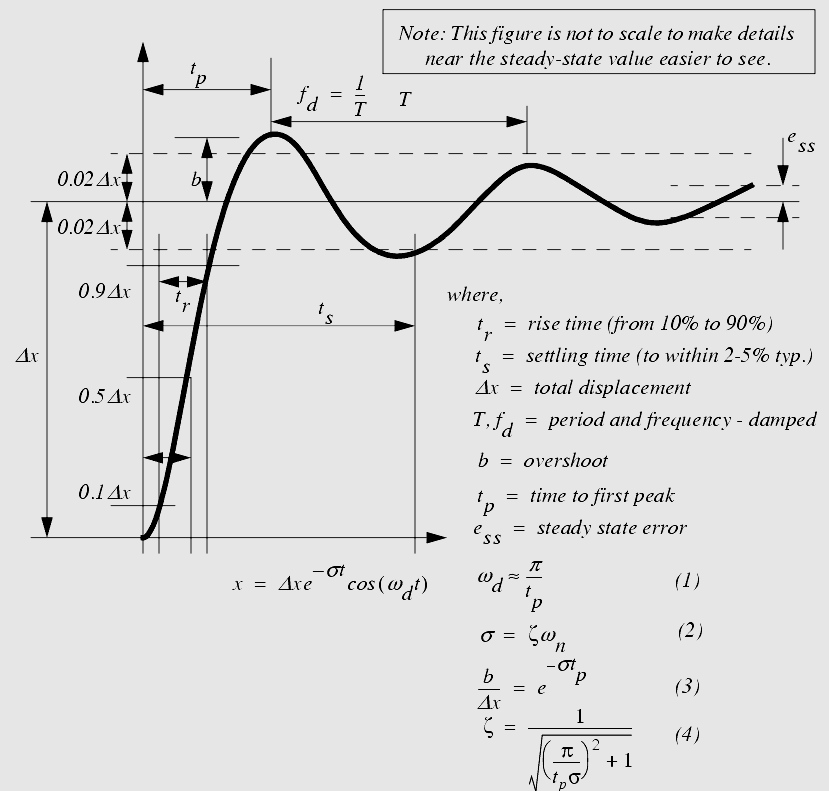
\includegraphics[width=\textwidth]{Images/2ndOrderTransient.png}
				2nd Order System Response \cite{engineerOnADisk_2ndOrderDynamics}
			\end{figure}
		\end{column}
	\end{columns}
\end{frame}

\section{Steady-state Forced Response}
\begin{frame}
	\frametitle{Review: Steady-state Input System Response}
	\begin{figure}
		\centering
		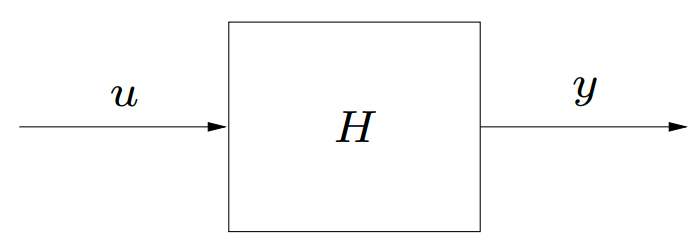
\includegraphics[width = 0.25\textwidth]{Images/H(s)_BlockDiagram.png}
	\end{figure}
	\textbf{Convolution:} 
	\[
		y(t) = \int_{0}^{t} h(\tau) u(t - \tau) \dd \tau 
		\quad 
		Y(s) = H(s) U(s)
	\]
	\textbf{Sinusoidal Input:} 
	\[
		u(t) = cos(\omega t) = (e^{j\omega t} + e^{-j\omega t})/2 = 1 e^{j 0}
	\]
	\textbf{Steady-State Output:} 
	\[
		y(t) = \int_{0}^{\infty} h(\tau) cos(\omega (t - \tau)) \dd \tau = A e^{j \phi} = A \cos(\omega t + \phi)
	\]
	where $A = \abs{H(j \omega)}$ and $\phi = \angle(H(j \omega))$.
\end{frame}


\begin{frame}
	\frametitle{Steady-state System Response}
	\begin{columns}
		\begin{column}{0.3\textwidth}
			\textbf{Magnitude Gain:} 
			\[\abs{H(j\omega)} = \frac{Y_0}{U_0} = \frac{1.5}{2} = 0.75\]
			\textbf{Phase Shift:}
			\[\angle{H(j\omega)} = \phi = \frac{\pi}{4}\]
		\end{column}
		\begin{column}{0.5\textwidth}
			\[
				\color{red}
				u(t) = U_0 \cos(\omega t)
				\quad
				\color{blue}
				y(t) = Y_0 \cos(\omega t + \phi)
			\]
			\begin{figure}
				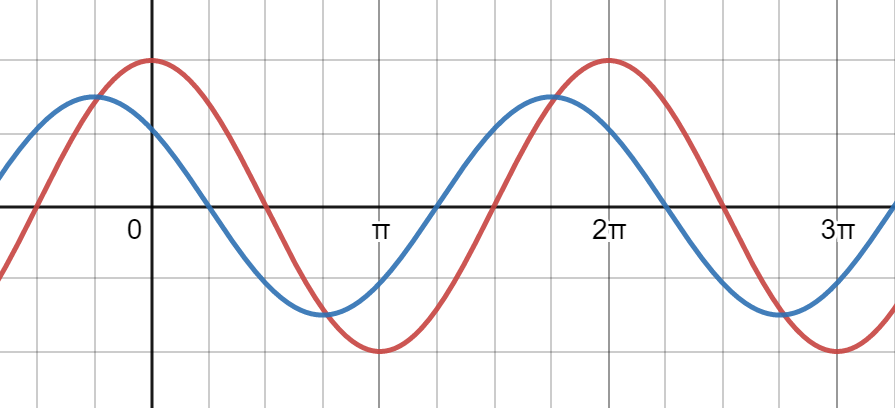
\includegraphics[width=\textwidth]{Images/phase_shift.png}
				Steady-state System Response with $\omega = 1$.
			\end{figure}
			\footnotesize{
				\textbf{Homework 6:}
				Sketch Bode Plots for given Transfer Functions
				\tiny{See posted review lectures for examples}
			}
		\end{column}
	\end{columns}
	\note{
		It is important to 
	}
\end{frame}

\section{Frequency Dependent Forced Response}
\begin{frame}
	\frametitle{Activity: Spring Mass Damper Frequency Response
	\cite{swarthmore_freq_response}}
	\begin{figure}
		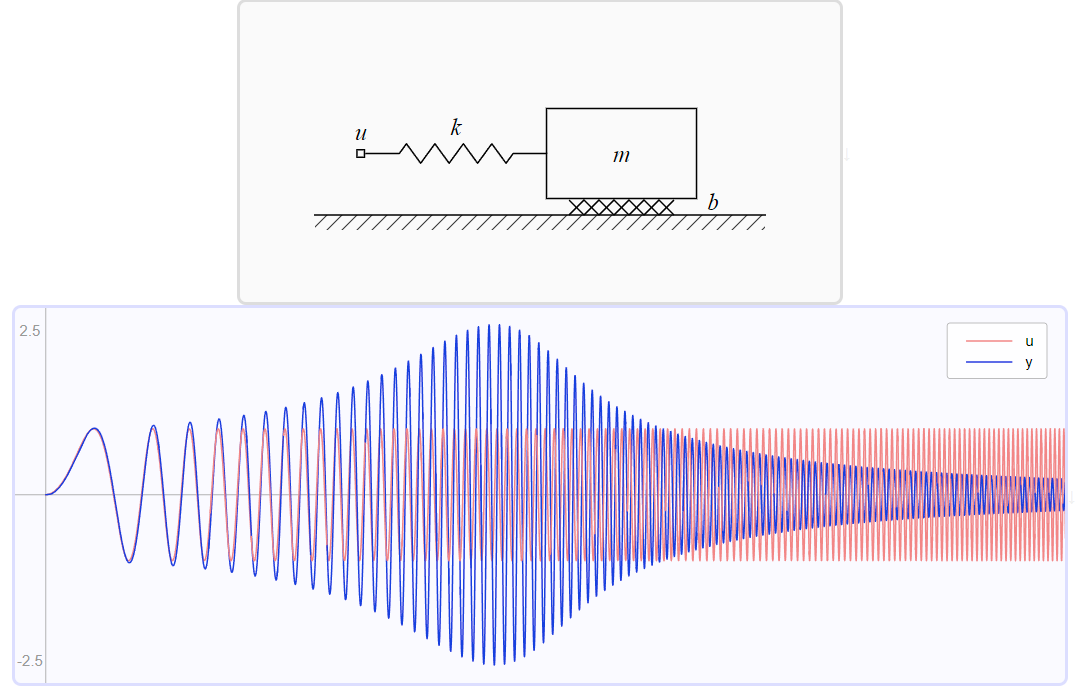
\includegraphics[width=0.625\textwidth]{Images/visualize_varied_freq_response.png}
		https://www.sccs.swarthmore.edu/users/12/abiele1/Linear/examples/freq.html
	\end{figure}
\end{frame}

\begin{frame}
	\frametitle{Bode Plot}
	\begin{columns}
		\begin{column}{0.375\textwidth}
			\textbf{Transfer Function:}
			\[
				H(s) 
				% = \cfrac{Y(s)}{U(s)} 
				= \cfrac{
					\omega_0^2
				}{
					s^2 + 2 \zeta \omega_0 s + \omega_0^2
				}
			\]
			\textbf{Magnitude Gain:} 
			\[\abs{H(j\omega)}_{db} = 20 \log_{10} \abs{\frac{Y_0}{U_0}}\]
			\textbf{Phase Shift:}
			\[\angle{H(j\omega)} = \phi\]
		\end{column}
		\begin{column}{0.5\textwidth}
			\begin{figure}
				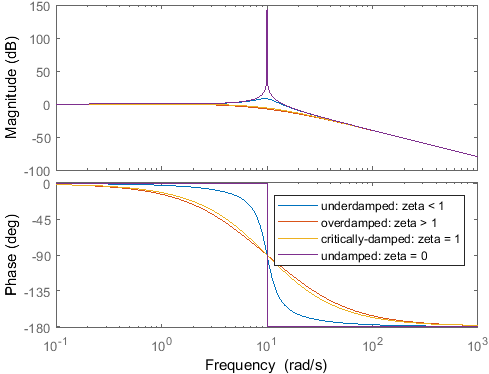
\includegraphics[width=\textwidth]{Images/bode_diagram.png}
				Bode Diagram varying dampening factor, $\zeta$.
			\end{figure}
		\end{column}
	\end{columns}
\end{frame}	

\begin{frame}
	\frametitle{Activity: Transfer Function Frequency Response}
	Investigate the system response by varying the input frequency, amplitude, and phase.
	{\cite{swarthmore_bode}}
	\begin{columns}
		\begin{column}{0.5\textwidth}
			\begin{figure}
				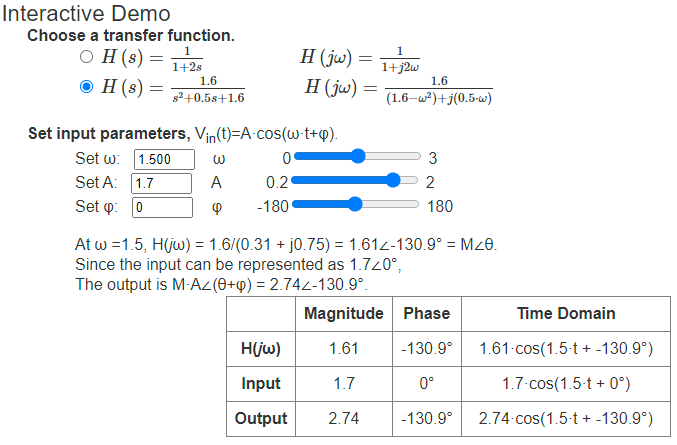
\includegraphics[width=\textwidth]{Images/bode_demo_1.png}
			\end{figure}
			\footnotesize{https://lpsa.swarthmore.edu/Bode/BodeWhat.html}
		\end{column}
		\begin{column}{0.4\textwidth}
			\begin{figure}
				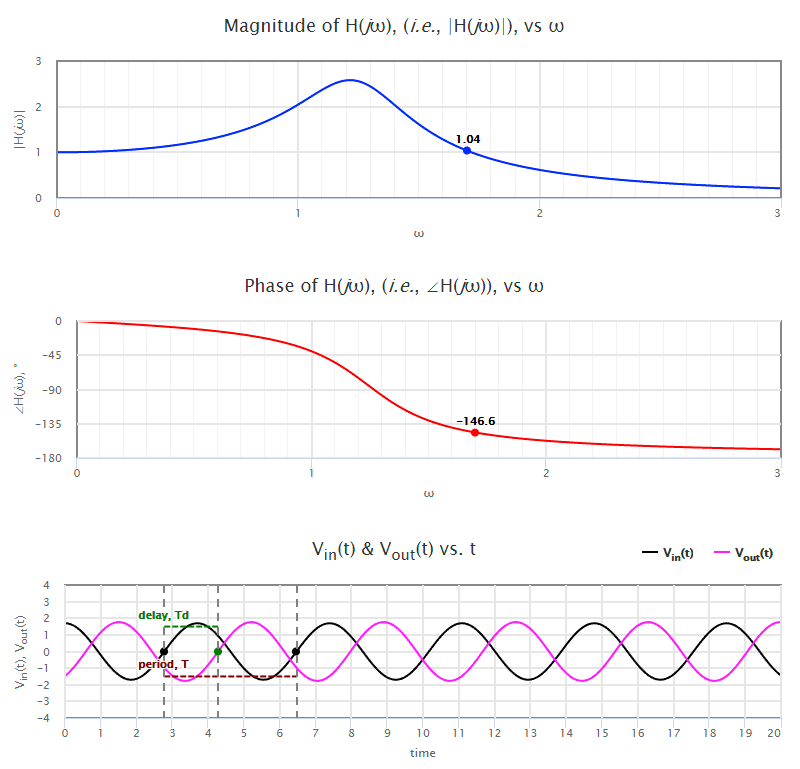
\includegraphics[width=\textwidth]{Images/bode_demo_2.png}
			\end{figure}
		\end{column}
	\end{columns}
\end{frame}

\section{Frequency Response System Characterization}
\begin{frame}
	\frametitle{Real-World Applications: System Characterization}
	\begin{columns}
		\begin{column}{0.375\textwidth}
			\centering
			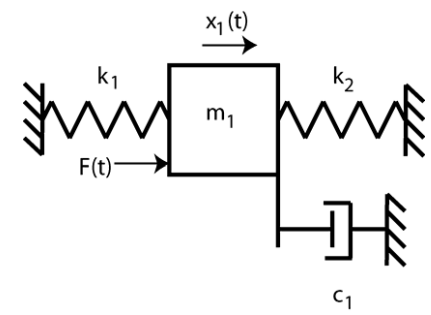
\includegraphics[width=0.75\textwidth]{Images/sys_char_diagram.png}\\
			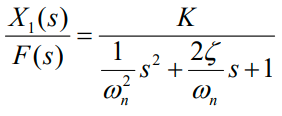
\includegraphics[width=0.5\textwidth]{Images/sys_char_tf.png}\\
			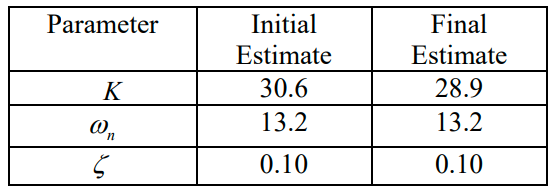
\includegraphics[width=\textwidth]{Images/sys_char_results.png}\\
			\footnotesize{System Characterization Paper Results 
			\cite{freq_response_charectorization}}
		\end{column}
		\begin{column}{0.5\textwidth}
			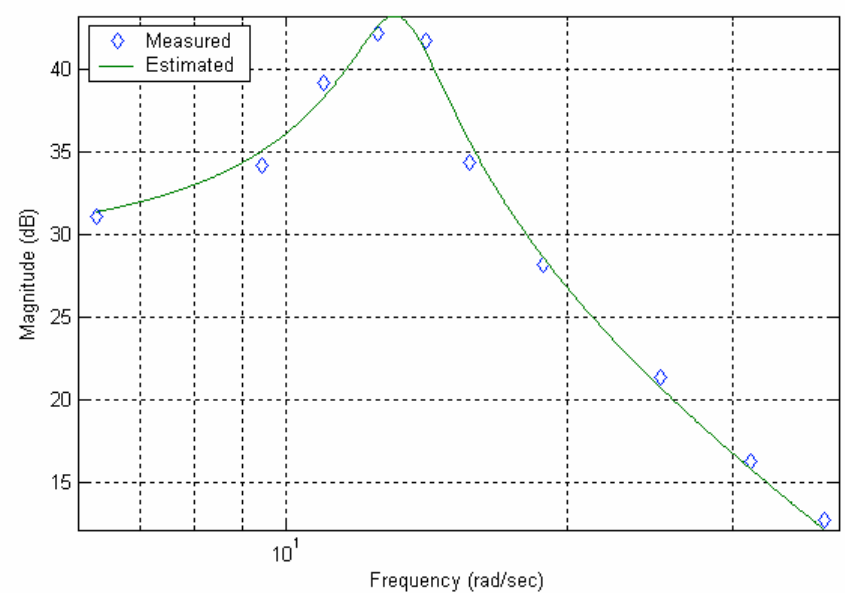
\includegraphics[width=\textwidth]{Images/sys_char_bode_data.png}
			\footnotesize{
				\textbf{Lab 3:}
				Experiment with selected system to obtain frequency response and characterize dynamics with an appropriate transfer function.
				\tiny{See lab instructions for more details}
				}
		\end{column}
	\end{columns}
\end{frame}

\section*{}

\begin{frame}
	\frametitle{Lecture Overview}
	\begin{columns}
		\begin{column}{0.25\textwidth}
			\[
				H(s)
				= \frac{
					\omega_0^2
				}{
					s^2 + 2 \zeta \omega_0 s + \omega_0^2
				}
			\]
			\[
				\omega_0 = \sqrt{\frac{k}{m}}
				\quad
				\zeta = \sqrt{\frac{c^2}{4 m k}}
			\]
			\begin{figure}[]
				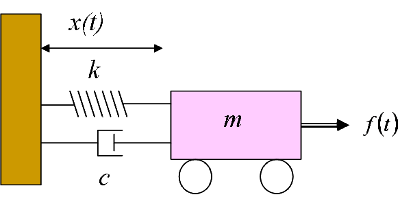
\includegraphics[width=\textwidth]{Images/SpringMassDamper_cartSystem.png}
			\end{figure}
		\end{column}
		\begin{column}{0.3\textwidth}
			\[
				\color{red}
				u(t) = U_0 \cos(\omega t)
			\]
			\[
				\color{blue}
				y(t) = Y_0 \cos(\omega t + \phi)
			\]
			\begin{figure}
				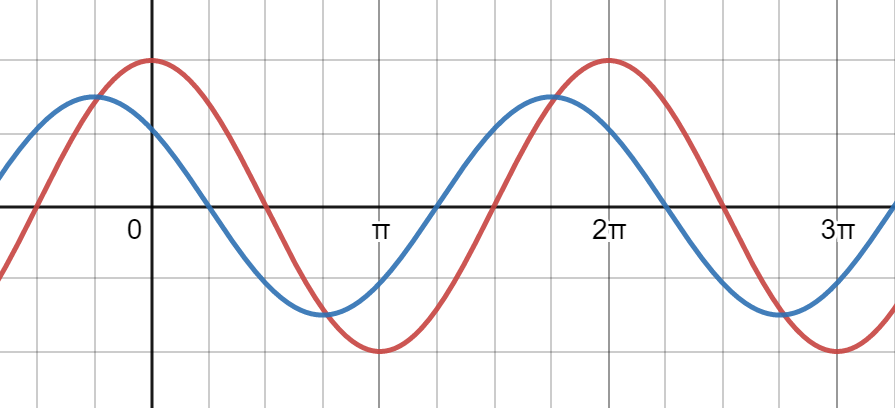
\includegraphics[width=\textwidth]{Images/phase_shift.png}
			\end{figure}
		\end{column}
		\begin{column}{0.4\textwidth}
			\begin{figure}
				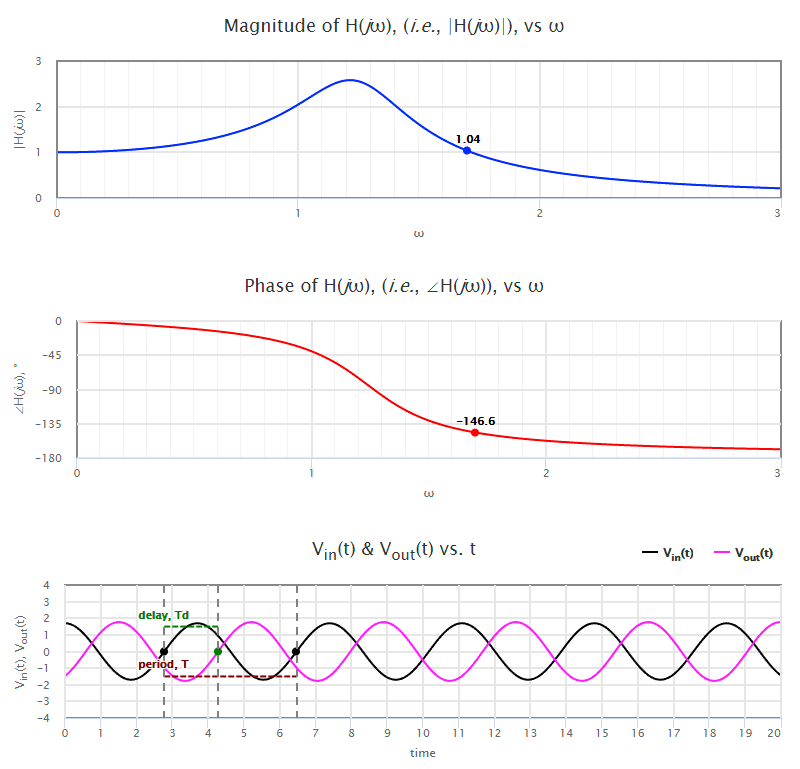
\includegraphics[width=\textwidth]{Images/bode_demo_2.png}
			\end{figure}
		\end{column}
	\end{columns}
\end{frame}

\begin{frame}[allowframebreaks]{Bibliography}
	\bibliographystyle{unsrt}
	\bibliography{refs}
\end{frame}


\end{document}